% Options for packages loaded elsewhere
\PassOptionsToPackage{unicode}{hyperref}
\PassOptionsToPackage{hyphens}{url}
\PassOptionsToPackage{dvipsnames,svgnames,x11names}{xcolor}
%
\documentclass[
  11pt,
  a4paper,
  DIV=11,
  numbers=noendperiod]{scrartcl}

\usepackage{amsmath,amssymb}
\usepackage{iftex}
\ifPDFTeX
  \usepackage[T1]{fontenc}
  \usepackage[utf8]{inputenc}
  \usepackage{textcomp} % provide euro and other symbols
\else % if luatex or xetex
  \usepackage{unicode-math}
  \defaultfontfeatures{Scale=MatchLowercase}
  \defaultfontfeatures[\rmfamily]{Ligatures=TeX,Scale=1}
\fi
\usepackage{lmodern}
\ifPDFTeX\else  
    % xetex/luatex font selection
\fi
% Use upquote if available, for straight quotes in verbatim environments
\IfFileExists{upquote.sty}{\usepackage{upquote}}{}
\IfFileExists{microtype.sty}{% use microtype if available
  \usepackage[]{microtype}
  \UseMicrotypeSet[protrusion]{basicmath} % disable protrusion for tt fonts
}{}
\makeatletter
\@ifundefined{KOMAClassName}{% if non-KOMA class
  \IfFileExists{parskip.sty}{%
    \usepackage{parskip}
  }{% else
    \setlength{\parindent}{0pt}
    \setlength{\parskip}{6pt plus 2pt minus 1pt}}
}{% if KOMA class
  \KOMAoptions{parskip=half}}
\makeatother
\usepackage{xcolor}
\usepackage[lmargin=2cm,rmargin=2cm,tmargin=2cm,bmargin=2cm]{geometry}
\setlength{\emergencystretch}{3em} % prevent overfull lines
\setcounter{secnumdepth}{-\maxdimen} % remove section numbering
% Make \paragraph and \subparagraph free-standing
\ifx\paragraph\undefined\else
  \let\oldparagraph\paragraph
  \renewcommand{\paragraph}[1]{\oldparagraph{#1}\mbox{}}
\fi
\ifx\subparagraph\undefined\else
  \let\oldsubparagraph\subparagraph
  \renewcommand{\subparagraph}[1]{\oldsubparagraph{#1}\mbox{}}
\fi


\providecommand{\tightlist}{%
  \setlength{\itemsep}{0pt}\setlength{\parskip}{0pt}}\usepackage{longtable,booktabs,array}
\usepackage{calc} % for calculating minipage widths
% Correct order of tables after \paragraph or \subparagraph
\usepackage{etoolbox}
\makeatletter
\patchcmd\longtable{\par}{\if@noskipsec\mbox{}\fi\par}{}{}
\makeatother
% Allow footnotes in longtable head/foot
\IfFileExists{footnotehyper.sty}{\usepackage{footnotehyper}}{\usepackage{footnote}}
\makesavenoteenv{longtable}
\usepackage{graphicx}
\makeatletter
\def\maxwidth{\ifdim\Gin@nat@width>\linewidth\linewidth\else\Gin@nat@width\fi}
\def\maxheight{\ifdim\Gin@nat@height>\textheight\textheight\else\Gin@nat@height\fi}
\makeatother
% Scale images if necessary, so that they will not overflow the page
% margins by default, and it is still possible to overwrite the defaults
% using explicit options in \includegraphics[width, height, ...]{}
\setkeys{Gin}{width=\maxwidth,height=\maxheight,keepaspectratio}
% Set default figure placement to htbp
\makeatletter
\def\fps@figure{htbp}
\makeatother

\KOMAoption{captions}{tableheading}
\makeatletter
\@ifpackageloaded{caption}{}{\usepackage{caption}}
\AtBeginDocument{%
\ifdefined\contentsname
  \renewcommand*\contentsname{Table of contents}
\else
  \newcommand\contentsname{Table of contents}
\fi
\ifdefined\listfigurename
  \renewcommand*\listfigurename{List of Figures}
\else
  \newcommand\listfigurename{List of Figures}
\fi
\ifdefined\listtablename
  \renewcommand*\listtablename{List of Tables}
\else
  \newcommand\listtablename{List of Tables}
\fi
\ifdefined\figurename
  \renewcommand*\figurename{Figure}
\else
  \newcommand\figurename{Figure}
\fi
\ifdefined\tablename
  \renewcommand*\tablename{Table}
\else
  \newcommand\tablename{Table}
\fi
}
\@ifpackageloaded{float}{}{\usepackage{float}}
\floatstyle{ruled}
\@ifundefined{c@chapter}{\newfloat{codelisting}{h}{lop}}{\newfloat{codelisting}{h}{lop}[chapter]}
\floatname{codelisting}{Listing}
\newcommand*\listoflistings{\listof{codelisting}{List of Listings}}
\makeatother
\makeatletter
\makeatother
\makeatletter
\@ifpackageloaded{caption}{}{\usepackage{caption}}
\@ifpackageloaded{subcaption}{}{\usepackage{subcaption}}
\makeatother
\ifLuaTeX
  \usepackage{selnolig}  % disable illegal ligatures
\fi
\usepackage{bookmark}

\IfFileExists{xurl.sty}{\usepackage{xurl}}{} % add URL line breaks if available
\urlstyle{same} % disable monospaced font for URLs
\hypersetup{
  pdftitle={Uluslararası Göç İstatistikleri Analizi},
  colorlinks=true,
  linkcolor={blue},
  filecolor={Maroon},
  citecolor={Blue},
  urlcolor={Blue},
  pdfcreator={LaTeX via pandoc}}

\title{Uluslararası Göç İstatistikleri Analizi}
\author{}
\date{}

\begin{document}
\maketitle

\section[{1. Amaç ve Kapsam} ]{\texorpdfstring{{1. Amaç ve Kapsam}
\protect
\includegraphics[width=0.23958in,height=0.23958in]{images/clipboard-3134960358.png}}{1. Amaç ve Kapsam }}\label{amauxe7-ve-kapsam}

\begin{itemize}
\item
  Türkiye'nin maruz kaldığı uluslararası göç hareketliliğinin büyüklük
  ve nitelik açısından analiz edilmesi
\item
  Yüksekokul ve üzeri eğitime sahip kişi sayısı ile göç sayısı
  arasındaki ilişkinin tespiti
\item
  İl bazında Gayrisafi Yurt İçi Hasıla ile göç sayısı arasındaki
  ilişkinin tespiti
\item
  Net göç oranına göre illerin kümelenmesi
\end{itemize}

\section[{2. Veri} ]{\texorpdfstring{{2. Veri}
\protect
\includegraphics[width=0.23958in,height=0.23958in]{images/clipboard-442643652.png}}{2. Veri }}\label{veri}

\subsection{\texorpdfstring{{\emph{2.1. Veri
Kaynağı}}}{2.1. Veri Kaynağı}}\label{veri-kaynaux11fux131}

\begin{itemize}
\item
  {[}Türkiye İstatistik Kurumu Uluslararası Göç
  İstistikleri{]}(https://data.tuik.gov.tr/Bulten/Index?p=Uluslararasi-Goc-Istatistikleri-2022-49457)
\item
  {[}İl Bazında Gayrisafi Yurt İçi
  Hasıla{]}(https://data.tuik.gov.tr/Bulten/Index?p=Il-Bazinda-Gayrisafi-Yurt-Ici-Hasila-2022-45867)
\item
  {[}Göç İdaresi Başkanlığı Düzensiz Göç
  İstatistikleri{]}(https://www.goc.gov.tr/duzensiz-goc-istatistikler)
\end{itemize}

\subsection{\texorpdfstring{{\emph{2.2. Veriye
Bakış}}}{2.2. Veriye Bakış}}\label{veriye-bakux131ux15f}

Analiz için 2022 yılına ait;

\begin{itemize}
\item
  Yaş grubu ve cinsiyete göre Türkiye'ye gelen ve Türkiye'den giden göç
  nüfus sayısı,
\item
  İllere göre Türkiye'ye gelen ve Türkiye'den giden göç nüfus sayısı,
\item
  Vatandaşlık ülkesine göre Türkiye'ye gelen ve Türkiye'den giden göç
  nüfus sayısı,
\item
  Türkiye'de vatandaşlık ülkesine göre yabancı uyruklu nüfus,
\item
  İller Bazında Gayrisafi Yurt İçi Hasıla(\$) verilerinden
  yararlanılacaktır.
\end{itemize}

\section[{3. Analiz} ]{\texorpdfstring{{3. Analiz}
\protect
\includegraphics[width=0.23958in,height=\textheight]{images/clipboard-355426313.png}}{3. Analiz }}\label{analiz}

Türkiye'deki mevcut durum tespit edilmiştir.

Zaman serisi analizi ile kaçak göçmen sayısının tahmini yapılmıştır.

Kümeleme ile göç oranına göre iller gruplandırılmıştır.

Regresyon analizi ile göç hareketliliği ile GSYH ve eğitim düzeyi
arasındaki ilişki belirlenmiştir.

\subsection{\texorpdfstring{\emph{3.1. Veri
Analizi}}{3.1. Veri Analizi}}\label{veri-analizi}

\subsubsection{\texorpdfstring{\emph{I) Cinsiyet ve Yaş Aralığı Bazında
Göç
Hareketliliği:}}{I) Cinsiyet ve Yaş Aralığı Bazında Göç Hareketliliği:}}\label{i-cinsiyet-ve-yaux15f-aralux131ux11fux131-bazux131nda-guxf6uxe7-hareketliliux11fi}

Cinsiyete göre hangi yaş aralığında daha yoğun göç hareketliliğinin
olduğu tespit edilmiştir.

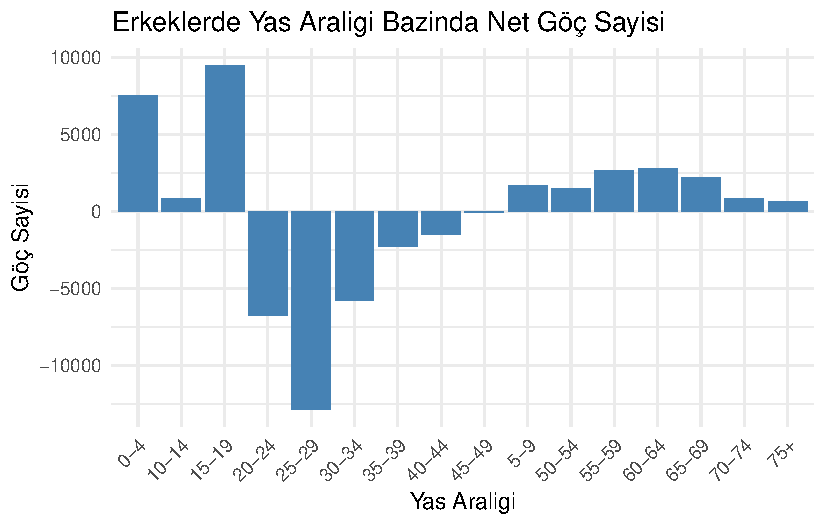
\includegraphics{project_files/figure-pdf/unnamed-chunk-2-1.pdf}

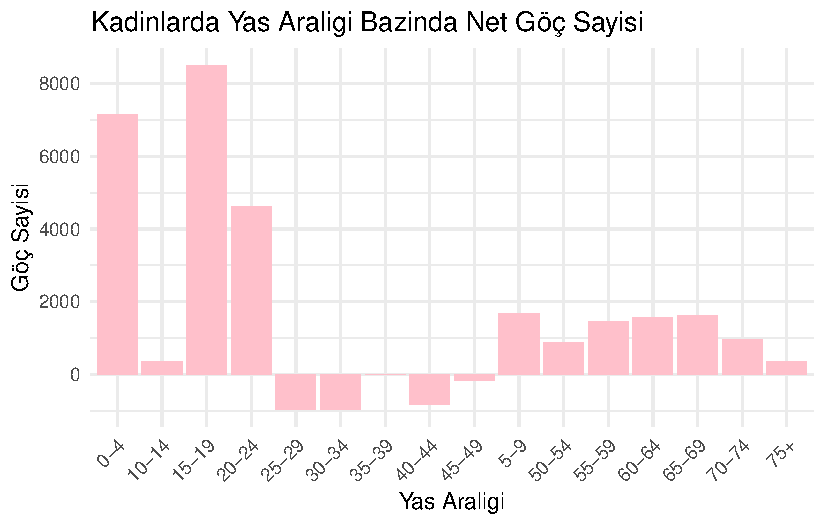
\includegraphics{project_files/figure-pdf/unnamed-chunk-3-1.pdf}

\subsubsection{\texorpdfstring{\emph{II) Yurt Dışına En Çok Göç Veren
Şehirler:}}{II) Yurt Dışına En Çok Göç Veren Şehirler:}}\label{ii-yurt-dux131ux15fux131na-en-uxe7ok-guxf6uxe7-veren-ux15fehirler}

Yurtdışına en çok göç veren ve yurtdışından en çok göç alan şehirler
belirlenmiştir. Bu şehirlerin nüfusuna oranla net göç oranı ortaya
konmuştur.

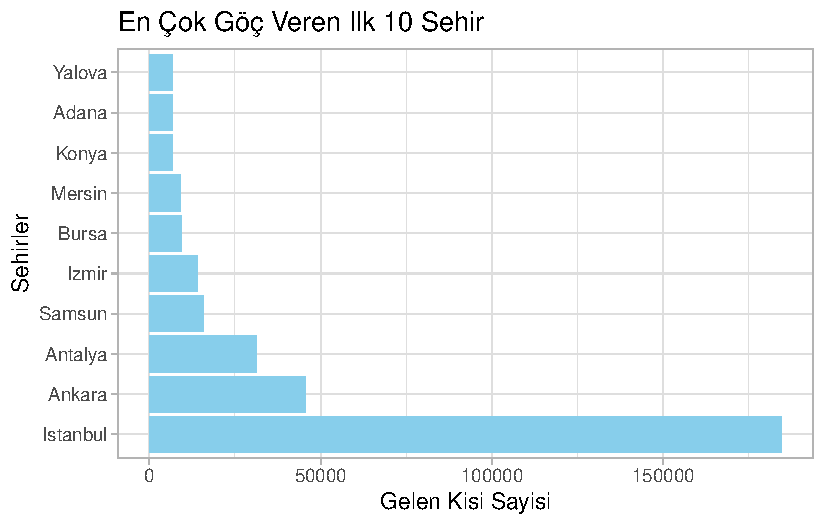
\includegraphics{project_files/figure-pdf/unnamed-chunk-4-1.pdf}

\subsubsection{\texorpdfstring{\emph{III)Yurt Dışından En Çok Göç Alan
Şehirler:}}{III)Yurt Dışından En Çok Göç Alan Şehirler:}}\label{iiiyurt-dux131ux15fux131ndan-en-uxe7ok-guxf6uxe7-alan-ux15fehirler}

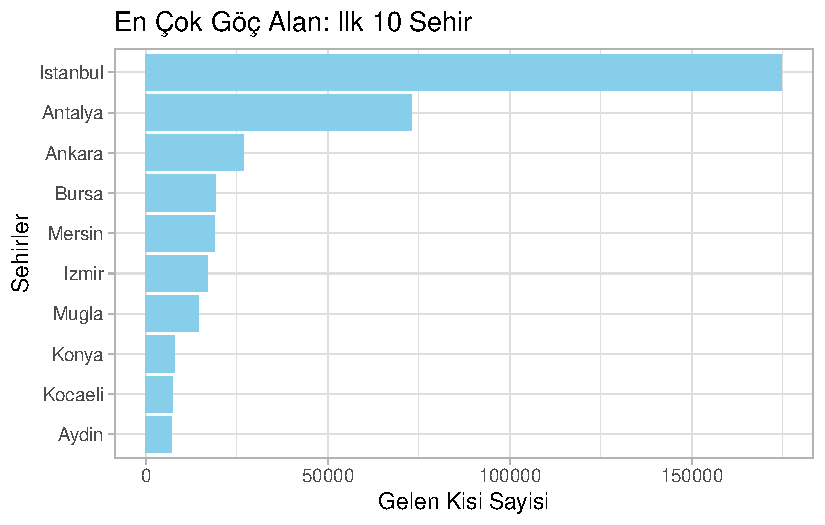
\includegraphics{project_files/figure-pdf/unnamed-chunk-5-1.pdf}

\subsubsection{\texorpdfstring{\emph{IV) İller Bazında Nüfusa Oranla Net
Göç
Oranı:}}{IV) İller Bazında Nüfusa Oranla Net Göç Oranı:}}\label{iv-iller-bazux131nda-nuxfcfusa-oranla-net-guxf6uxe7-oranux131}

\begin{verbatim}

Attaching package: 'dplyr'
\end{verbatim}

\begin{verbatim}
The following objects are masked from 'package:stats':

    filter, lag
\end{verbatim}

\begin{verbatim}
The following objects are masked from 'package:base':

    intersect, setdiff, setequal, union
\end{verbatim}

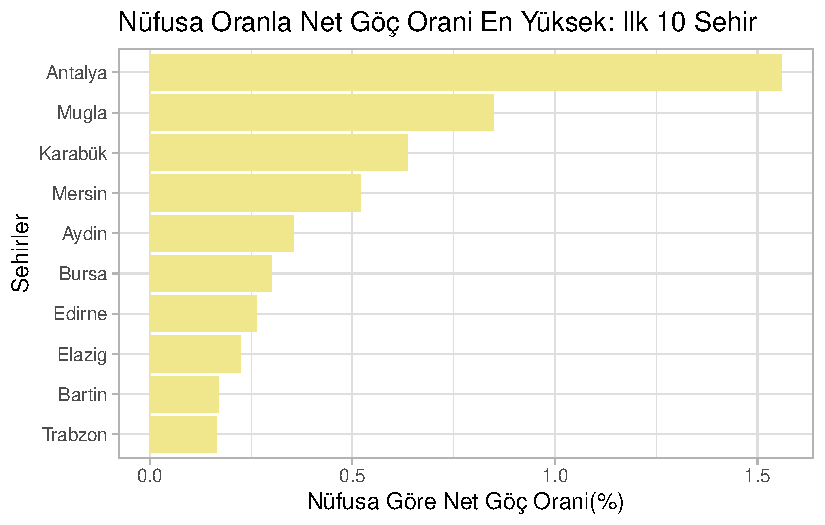
\includegraphics{project_files/figure-pdf/unnamed-chunk-6-1.pdf}

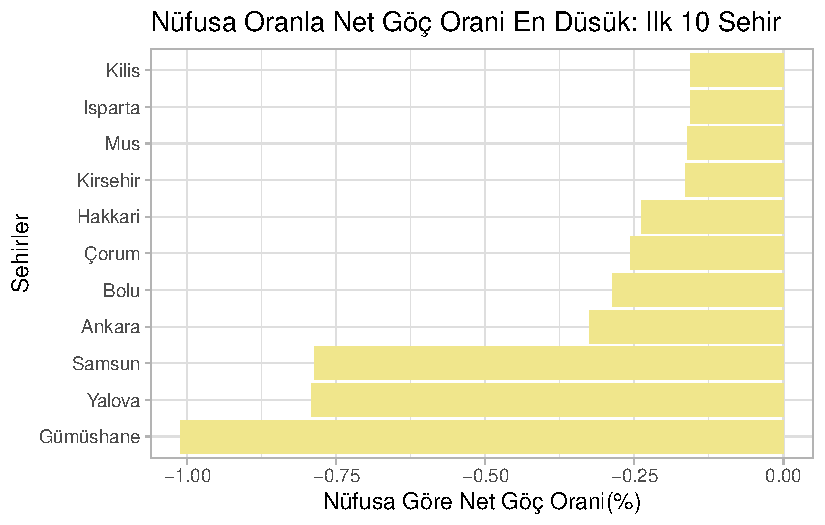
\includegraphics{project_files/figure-pdf/unnamed-chunk-6-2.pdf}

\subsubsection{\texorpdfstring{\emph{V) Ülkeler Bazında Göç
Dağılımı:}}{V) Ülkeler Bazında Göç Dağılımı:}}\label{v-uxfclkeler-bazux131nda-guxf6uxe7-daux11fux131lux131mux131}

Yurtdışından en çok göç alınan ülkeler ve yurtdışına en çok edilen
ülkeler belirlenmiştir.

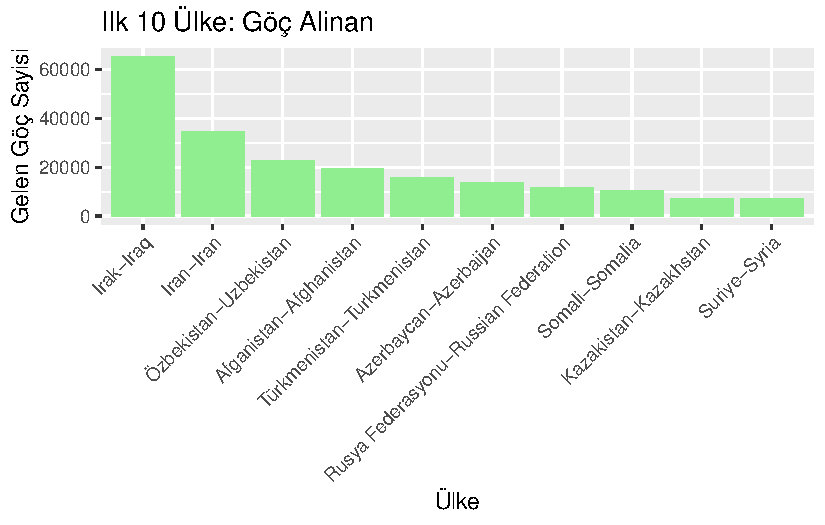
\includegraphics{project_files/figure-pdf/unnamed-chunk-7-1.pdf}

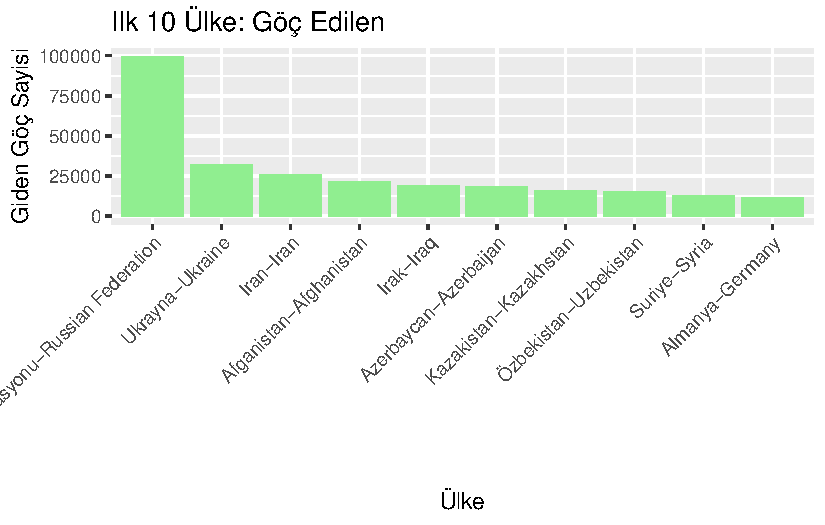
\includegraphics{project_files/figure-pdf/unnamed-chunk-7-2.pdf}

\subsubsection{\texorpdfstring{\emph{VI) Türkiye'deki Yabancı Uyruk
Nüfusu:}}{VI) Türkiye'deki Yabancı Uyruk Nüfusu:}}\label{vi-tuxfcrkiyedeki-yabancux131-uyruk-nuxfcfusu}

Ülkemizde yer alan yabancı uyruklu nüfus sayısı tespit edilmiştir.

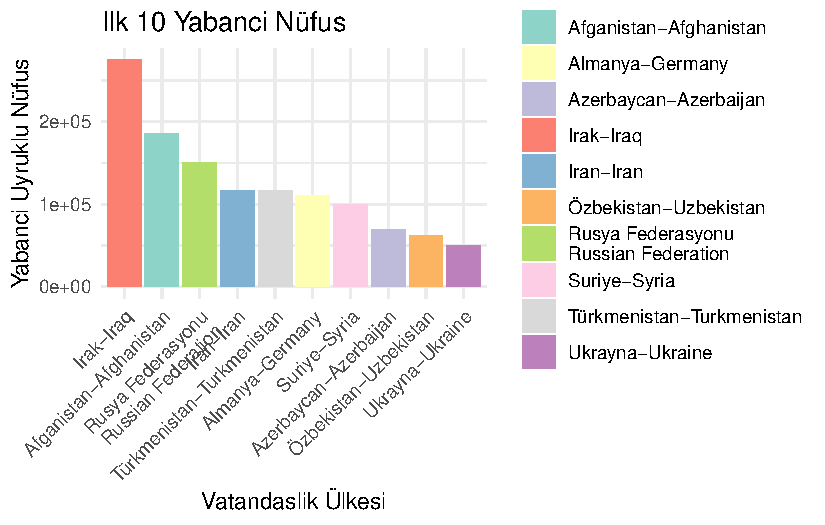
\includegraphics{project_files/figure-pdf/unnamed-chunk-8-1.pdf}

\subsubsection{\texorpdfstring{\emph{VII) İller Bazında Eğitim Düzeyi ve
Göç ArasındaKİ
İlişki:}}{VII) İller Bazında Eğitim Düzeyi ve Göç ArasındaKİ İlişki:}}\label{vii-iller-bazux131nda-eux11fitim-duxfczeyi-ve-guxf6uxe7-arasux131ndaki-iliux15fki}

Yüksekokul ve üzeri eğitim düzeyi ile yurtdışına yapılan göç arasındaki
ilişki ortaya konmuştur.

\begin{verbatim}

Call:
lm(formula = yuksekokul ~ giden, data = illeregoreegitim)

Residuals:
    Min      1Q  Median      3Q     Max 
-167685  -51531  -27370   16280  597463 

Coefficients:
             Estimate Std. Error t value Pr(>|t|)    
(Intercept) 6.996e+04  1.331e+04   5.255 1.22e-06 ***
giden       1.760e+01  6.121e-01  28.755  < 2e-16 ***
---
Signif. codes:  0 '***' 0.001 '**' 0.01 '*' 0.05 '.' 0.1 ' ' 1

Residual standard error: 115500 on 79 degrees of freedom
Multiple R-squared:  0.9128,    Adjusted R-squared:  0.9117 
F-statistic: 826.9 on 1 and 79 DF,  p-value: < 2.2e-16
\end{verbatim}

\begin{verbatim}
`geom_smooth()` using formula = 'y ~ x'
\end{verbatim}

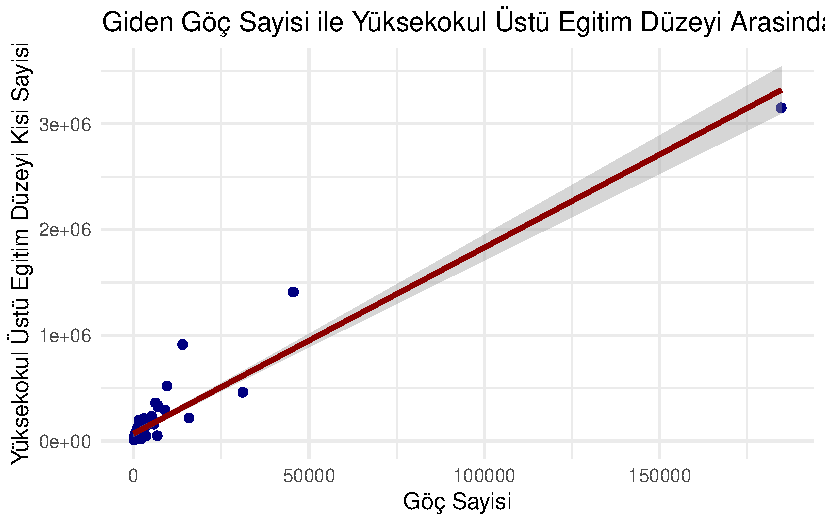
\includegraphics{project_files/figure-pdf/unnamed-chunk-9-1.pdf}

\subsubsection{\texorpdfstring{\emph{VIII) Uluslararası Göç İstatistiği
ile Gayrisafi Yurt İçi Hasıla Arasındaki
İlişki:}}{VIII) Uluslararası Göç İstatistiği ile Gayrisafi Yurt İçi Hasıla Arasındaki İlişki:}}\label{viii-uluslararasux131-guxf6uxe7-istatistiux11fi-ile-gayrisafi-yurt-iuxe7i-hasux131la-arasux131ndaki-iliux15fki}

iller bazında gayrisafi yurt içi hasıla tutarı ile net göç arasındaki
ilişki ortaya konmuştur.

\begin{verbatim}

Call:
lm(formula = GSYH ~ net, data = data)

Residuals:
    Min      1Q  Median      3Q     Max 
-4643.8 -2266.1  -617.2  1539.5 10289.8 

Coefficients:
             Estimate Std. Error t value Pr(>|t|)    
(Intercept) 7.943e+03  3.372e+02  23.559   <2e-16 ***
net         3.201e-02  5.877e-02   0.545    0.588    
---
Signif. codes:  0 '***' 0.001 '**' 0.01 '*' 0.05 '.' 0.1 ' ' 1

Residual standard error: 3029 on 79 degrees of freedom
Multiple R-squared:  0.00374,   Adjusted R-squared:  -0.008871 
F-statistic: 0.2965 on 1 and 79 DF,  p-value: 0.5876
\end{verbatim}

\begin{verbatim}
`geom_smooth()` using formula = 'y ~ x'
\end{verbatim}

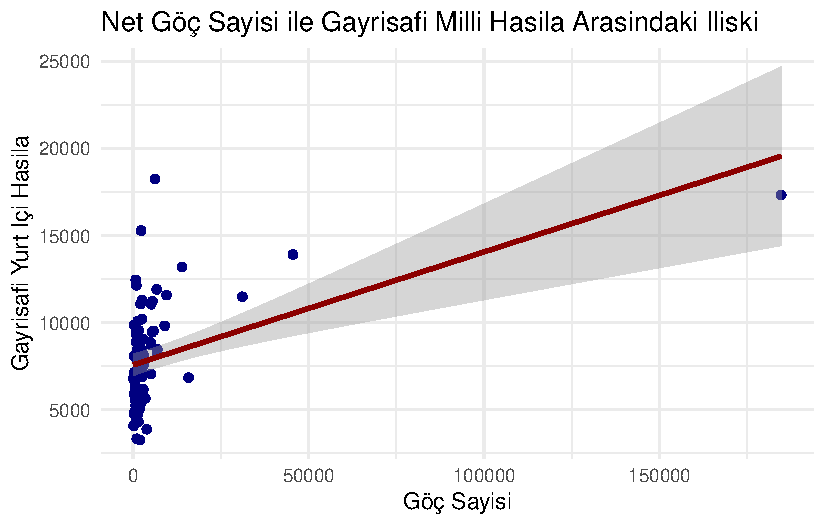
\includegraphics{project_files/figure-pdf/unnamed-chunk-10-1.pdf}

\subsubsection{\texorpdfstring{\emph{IX) Göç Oranına Göre İlleri
Kümeleme:}}{IX) Göç Oranına Göre İlleri Kümeleme:}}\label{ix-guxf6uxe7-oranux131na-guxf6re-illeri-kuxfcmeleme}

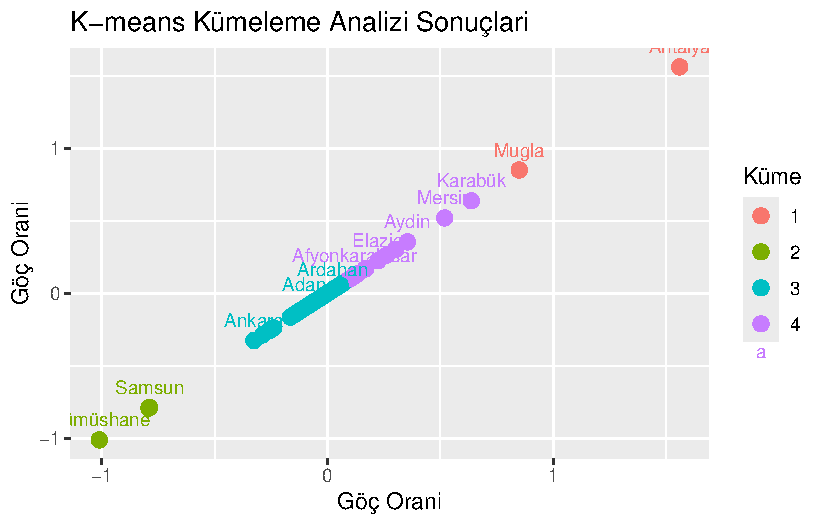
\includegraphics{project_files/figure-pdf/unnamed-chunk-11-1.pdf}

\section[{4. Sonuç ve Çıkarımlar} ]{\texorpdfstring{{4. Sonuç ve
Çıkarımlar}
\protect
\includegraphics[width=0.36458in,height=\textheight]{images/clipboard-1698656164.png}}{4. Sonuç ve Çıkarımlar }}\label{sonuuxe7-ve-uxe7ux131karux131mlar}

\begin{center}
\includegraphics[width=2.69792in,height=\textheight]{images/sonuc.gif}
\end{center}

Bu çalışma ile Türkiye'nin uluslararası göç istatistiklerinin cinsiyet,
yaş aralığı, vatandaşlık ülkesine göre mevcut durumu ortaya konmuştur.

Ülkemizden giden nüfusun eğitim düzeyi ile ilişkisi araştırılmıştır.
Yüksekokul ve üzeri eğitim düzeyine sahip kişilerin giden göç sayısıyla
ilişkili olduğu tespit edilmiştir.

Net göç sayısı ve Gayrisafi Yurt İçi Hasıla arasındaki ilişki
araştırılmıştır. GSYH ile net göç arasında bir lişki olmadığı tespit
edilmiştir.

Son olarak, göç oranına göre iller kümelenmiştir.



\end{document}
